\section{Space-Time Cube}\label{sec:impl-stc}
After the insertion of the data, the cube representation is run in the browser/viewer. Before the cube is presented, the list of the artists will
pop up, and the user needs to select those artists that they wish to visualize. This can either be a single artist, if only one life is to be
explored, or multiple artists if the connections between them are deemed important.

\begin{figure}[hbt!]
    \begin{center}
        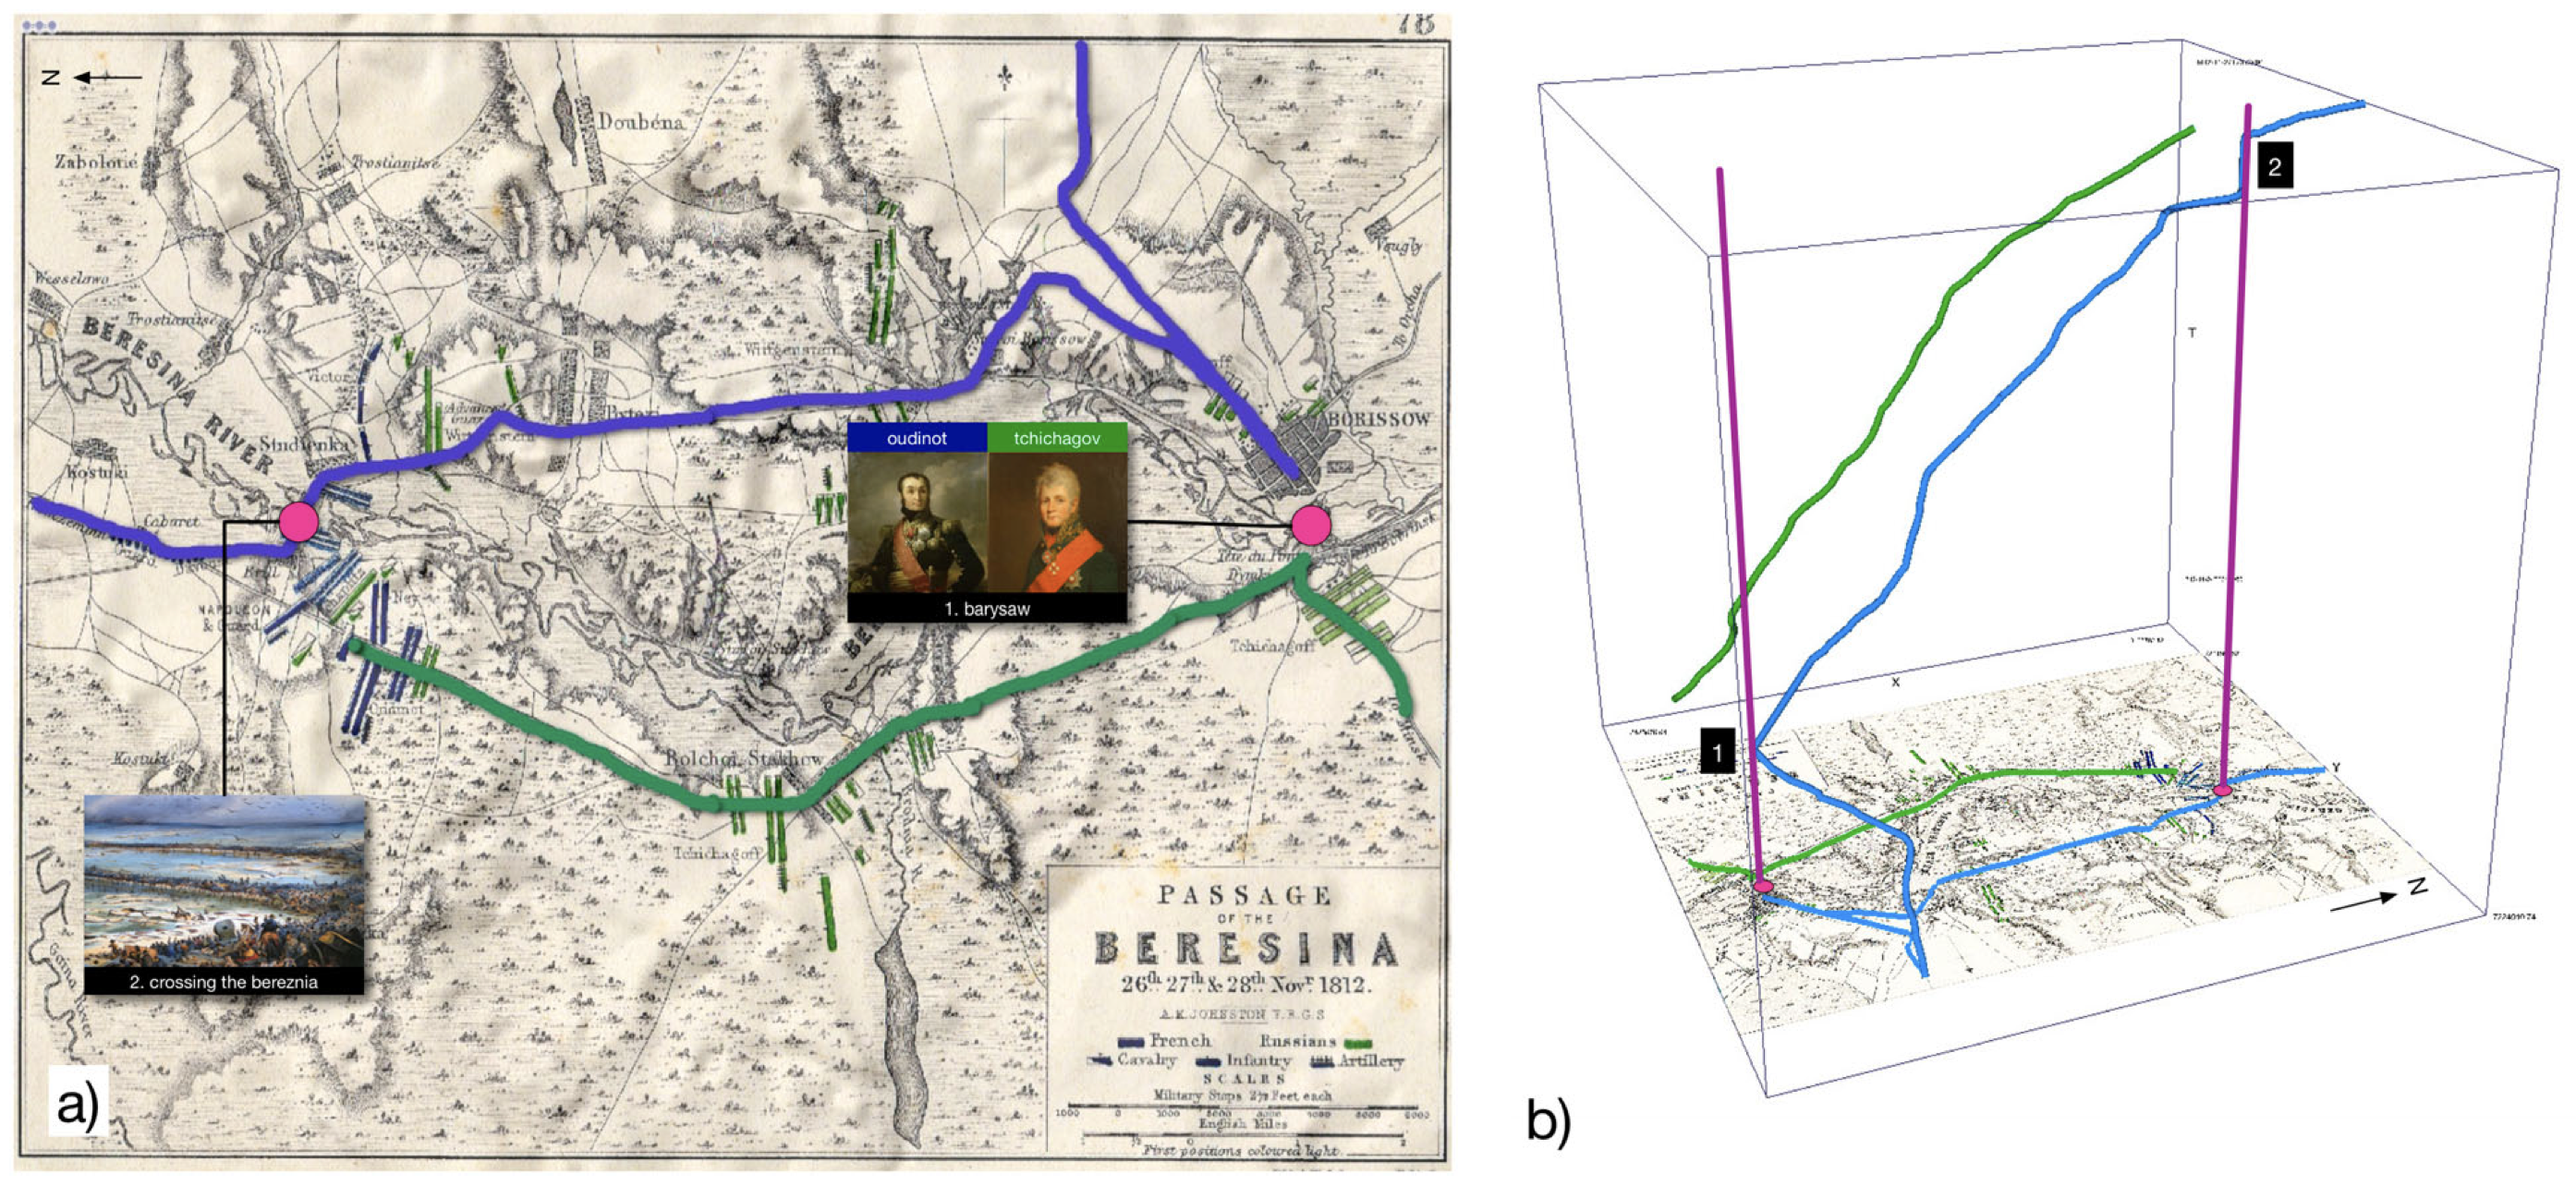
\includegraphics[width=\textwidth]{graphics/3-implementation/9}
    \end{center}
    \caption{Selection of artists for the visualization of the space-time cube}
    \label{fig:figure3.9}
\end{figure}

\subsection{3D Web Browser Version}\label{subsec:3d-version}
The first presentation of the space-time cube is the 3D web browser version. The cube uses two dimensions to
represent the spatial dimension, and the third one to represent time. On the bottom of the cube, the map is shown. It includes all the cities
that the artists lived in, represented with small dots on the map. The main element in the cube is the space-time path. It shows the artists'
lives trajectories. Vertical lines represent the stay in each city and the length of them depends on how long the stay
was. If the stay was marked as important, it is colored and labeled differently. The user can click
on these labels and read information about why the stay was important. Marking the stay as important and describing it was mentioned in
\Cref{sec:managing-artists}. The third dimension contains a timeline with year labels. These can be modified to show the whole date as well.

The toolbar gives us multiple filtering options related to a number of variables, among which are: seeing the artists' number of artworks,
connections to other artists, exhibitions and historic events. Each of the options is presented differently in the cube, using distinct labels,
and their meaning is explained in the toolbar. On the top of the page is a button which gives the user the possibility to switch to 2D mode. More
about this will be explained in \Cref{subsec:time-flattened-version}.

\begin{figure}[hbt!]
    \begin{center}
        \includegraphics[width=0.9\textwidth]{graphics/3-implementation/10}
    \end{center}
    \caption{Space-time cube visualization in a web browser}
    \label{fig:figure3.10}
\end{figure}

\clearpage

\subsection{Time-Flattened Browser Version}\label{subsec:time-flattened-version}
The other version of the visualization that can be presented in the browser is the time-flattened cube which shows only a two-dimensional map. This
operation of time flattening has been mentioned in \Cref{sec:space-time-cube} and seen in \Cref{fig:figure2.9}. The reason behind introducing
this option is to concentrate only on the spatial trajectory of the artist's life without giving full details about time (the trajectory depends on
time, but the temporal intervals are not explicit anymore). This way, artists' trajectories can be observed with a main focus on spatial
movement and some other aspects related to it.

\begin{figure}[hbt!]
    \begin{center}
        \includegraphics[width=0.8\textwidth]{graphics/3-implementation/11}
    \end{center}
    \caption{Time-flattened space-time cube}
    \label{fig:figure3.11}
\end{figure}

\clearpage

\subsection{General Technical Features of the Space-Time Cube}\label{subsec:technical-specifics-stc}
Before moving to the AR presentation, we discuss some details related to the implementation of the space-time cube.

\subsubsection{Generating the Timeline}

For generating the timeline for our representation of the cube, at least two years are needed to be used as the initial and end year. The cube
takes the list of selected artists. It then looks at where and when the artists lived, to determine the initial and the final years any of the
selected artis lived in. In the coordinate system of Three.js, the initial year should be mapped to the $y=-0.5$ coordinate, since this is the
lowest point of the cube. Similarly, the final year should be mapped to the $y=0.5$ coordinate. This concept is illustrated in the figure below.

\vspace{0.5cm}

\begin{figure}[hbt!]
    \begin{center}
        \begin{tikzpicture}
            \draw[-] (-3.0,0) -- (3.0,0) ; %edit here for the axis
            \draw[gray,dashed,->] (-3, -0.7) -- (-3, -1.7);
            \draw[gray,dashed,->] (3, -0.7) -- (3, -1.7);

            \draw[shift={(-3,0)},color=black] (0pt,3pt) -- (0pt,-3pt);
            \draw[shift={(3,0)},color=black] (0pt,3pt) -- (0pt,-3pt);

            \draw[shift={(-3,0)},color=black] (0pt,0pt) -- (0pt,-3pt) node[below]
                {$1980$};
            \draw[shift={(3,0)},color=black] (0pt,0pt) -- (0pt,-3pt) node[below]
                {$2000$};

            \draw[-] (-3.0,-2) -- (3.0,-2) ; %edit here for the axis
            \draw[shift={(-3,-2)},color=black] (0pt,3pt) -- (0pt,-3pt);
            \draw[shift={(3,-2)},color=black] (0pt,3pt) -- (0pt,-3pt);

            \draw[shift={(-3,-2)},color=black] (0pt,0pt) -- (0pt,-3pt) node[below]
                {$-0.5$};
            \draw[shift={(3,-2)},color=black] (0pt,0pt) -- (0pt,-3pt) node[below]
                {$0.5$};
        \end{tikzpicture}
    \end{center}
    \caption{Mapping of years in the space-time cube}
    \label{fig:figure3.12}
\end{figure}

Naturally, we can achieve the desired result using a linear mapping. Let $m$ be the minimum year and $M$ be the maximum year. Then, the following
function can be used to map any year $y$ to the range $[-0.5,\ 0.5]$:

\begin{align*}
    f(y) = \frac{y - m}{M - m} - \frac 12
\end{align*}

Additionally, mapping the earliest and the latest years to the edges of the cube is not visually pleasing. Because of this, a small padding of a
few years is added to both minimum and the maximum year before defining the function $f$ so that the real minimum and maximum year values appear a
bit further away from the edge.

\clearpage

\subsubsection{Placing the Cities}

As we mentioned in \Cref{sec:managing-cities}, the whole map is not presented in the cube, only the portion which contains cities that the
selected artists lived in. However, when the cube receives the information about the cities in which the artists lived from the backend,
the coordinates of those cities are relative to the positions on the original map. These coordinates need to be adjusted to the cropped portion of
the map to retain the correct positions. In order to achieve this, the backend sends the coordinates of the upper-left and the bottom-right corners
of the cropped map relative to the original map. Based on this, we can create a mapping algorithm that maps the coordinates of the original map to
the coordinates of the cropped map.

The figure below presents the mapping and is followed by a detailed explanation.

\begin{figure}[hbt!]
    \begin{center}
        \begin{tikzpicture}
            \draw[-] (-5, -5) -- (-5, 5);
            \draw[-] (-5, 5) -- (5, 5);
            \draw[-] (5, -5) -- (5, 5);
            \draw[-] (-5, -5) -- (5, -5);
            %
            \draw[dashed] (-3, -3) -- (-3, 3);
            \draw[dashed] (-3, 3) -- (3, 3);
            \draw[dashed] (3, -3) -- (3, 3);
            \draw[dashed] (-3, -3) -- (3, -3);
            %
            \draw[dotted] (-1, 3) -- (-1, 0);
            \draw[dotted] (-3, 0) -- (-1, 0);
            %
            \node[] at (-5, 5.2) {\footnotesize $(0.0,0.0)$};
            \node[] at (5, -5.2) {\footnotesize $(1.0,1.0)$};
            %
            \node[] at (-3, 3.2) {\footnotesize $(0.2,0.2) \mapsto (0.0, 0.0)$};
            \node[] at (3, -3.2) {\footnotesize $(0.8,0.8) \mapsto (1.0, 1.0)$};
            \node[] at (-1, -0.2) {\footnotesize $(0.4,0.5) \mapsto (0.\overline 3,0.5)$};
            %
            \node at (-1,0) [circle,fill,inner sep=1.5pt]{};
        \end{tikzpicture}
    \end{center}
    \caption{Mapping the coordinates of the cities}
    \label{fig:figure3.13}
\end{figure}

As seen in \Cref{fig:figure3.13}, the upper-left corner of the original map which is presented as the outer square, has the coordinates
$(0.0,\ 0.0)$, whereas the lower-right one has the coordinates $(1.0,\ 1.0)$. If we want to map the coordinates $(0.4,\ 0.5)$ from the original
map to the cropped one, this can be again achieved by linear mapping. This mapping needs to map the upper-left and the lower-right corner of the
new map to the coordinates $(0.0,\ 0.0)$ and $(1.0,\ 1.0)$, respectively. Note that the original map is not necessarily square-shaped, so the
mapping function needs to be defined separately for $x$ and $y$ coordinates.

Let $m$ be the minimum value of one axis and $M$ be the maximum value of the same axis. Then, the following function can be defined to map the
coordinates $C$ from the original map to the cropped one:

\begin{align*}
    f(C) = \frac{C - m}{M - m}
\end{align*}

As seen in \Cref{fig:figure3.13}, the coordinates $(0.4,\ 0.5)$ from the original map are mapped to the coordinates $(0.\overline 3,\ 0.5)$ of the
cropped map.

\subsection{Technical Features of the Web Browser Version}\label{subsec:technical-specifics-browser-version}

In this section we will present some aspects of the representation of the space-time cube which are specific to the browser version of the
visualization.

\subsubsection{Switching Perspectives}

The initial visualization shown to the user is the three-dimensional cube. We already mentioned that this can be changed to the two-dimensional map
by clicking the ``Switch to 2D Mode'' button. The 3D version of the visualization should be presented using perspective projection to imitate how
the human eyes see. For this, the \texttt{PerspectiveCamera} is used.

In 2D mode, we want all the objects, no matter how distant from the camera, to stay the same size, and the lines which are parallel should be seen
as parallel. This means that the \texttt{PerspectiveCamera} can no longer be used, and so the \texttt{OrthographicCamera} needs to be used to
achieve this. Fortunately, Three.js allows a seamless switch between perspective and orthographic cameras for rendering the scene.

As said, the cube shows all the created objects inside it, but the 2D mode only shows the trajectory and the cities on the map. The rest of the
objects(timeline, residence labels, etc.) are hidden to avoid information cluttering.

\subsubsection{Interactivity}
The browser representation can be interactively manipulated by the user with the mouse and keyboard. The user can rotate or pan the camera and
zoom it in and out. Clicking on labels and certain objects for retrieving information is possible as well. However, the mouse cursor operates on a
2D surface, while the cube is a 3D object projected on a 2D plane. Because of this, the camera needs to be taken into
consideration as well. The technique which is applied here is called \emph{raycasting}. The idea is to imagine a ray which is fired from the camera
position and goes through the current cursor position on the screen, and to see if that ray intersects some relevant object in the 3D space. Such a
ray is fired for every frame of the render and the first object it goes through is saved in a variable. If the ray does not go through any relevant
object, the variable value is deleted. Then, when the left mouse button is clicked, we say that any object found in the variable is considered
clicked. This concept is also shown in the code below, \Cref{fig:3.14}.

\begin{figure}[hbt!]
    \begin{center}
        \begin{lstlisting}[language=JavaScript,label={lst:impl-stc-code-1},belowskip=-1 \baselineskip]
raycaster.setFromCamera(this.mouse, cube.camera);
const intersection = raycaster.intersectObjects(cube.castTargets);

if (intersection.length === 0) {
  this.selectedObject = null;
} else {
  this.selectedObject = intersection[0].object;
}
        \end{lstlisting}
    \end{center}
    \caption{Raycasting code example}
    \label{fig:3.14}
\end{figure}

% raycasting to click an object
% orbiting with the mouse and keyboard is also supported

\clearpage